%% ID: bathysphere
%% TITLE: Deep-sea submersible
%% TYPE: question
%% QUESTIONTYPE:  scq
%% CONCEPTS: forces, vectors1, trig
%% VIDEOS: 
%% LEVEL: 5
%% TOPIC: mechanics/statics
%% ORDER: 2

\begin{problem}[HSC1932PIIQ4a] % a harder statics problem, nice because it considers the idea of stable / unstable equilibrium, reworked to be multiple choice
 {\exposition{A bathysphere is a spherical deep-sea submersible which is lowered into the sea on a long cable. It's shell can be made thick enough to withstand depths over \quantity{1,000}{m}. It can be modelled as a spherical shell with a small window of very thick glass, which can be considered as a point mass.}
 
 \question{Before being lowered the bathysphere is floating on the surface, half submerged, by considering the angle of the window to the vertical and the potential energy of the whole system, which of the following is true:}   
   \begin{enumerate}
   \item \choice[a]{There are no points of equilibrium}
   \item \choice[b]{There is one point of equilibrium, which is unstable}
   \item \choice[c]{There is one point of equilibrium, which is stable}
   \item \choice[d]{There are two points of equilibrium, only one is stable}\correct
   \item \choice[e]{there are two points of equilibrium, both are stable}
   \end{enumerate}
   }
{\textit{Used with permission from UCLES, Higher School Certificate Physics, June 1932, Paper 2, Question 4.}}
{\answer{The correct answer is (d).}

As the mass of the shell is constant throughout and the amount of water displaced is unchanged by orientation of the shell (i.e. the bathysphere is spherically symmetric) can ignore the effect of the shell's mass and the mass of the water displaced.

Let the position of the window, which will be of mass $m$, be at an angle to the vertical, $\theta$ and label the radius of the sphere $r$. See Figure \ref{fig:Statics_Mercury_Balloon_1}.\\
\\This gives us a height, $h$, above the water, hence allowing us to equate the total potential energy, $V$, to the gravitational potential, which is given by $mgh$: \\

\begin{figure}
	\centering
	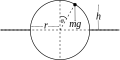
\includegraphics[width=0.4\textwidth]{Statics_Mercury_Balloon_1}
	\caption{}	
	\label{fig:Statics_Mercury_Balloon_1}
\end{figure}

Let the potential energy, $V(\theta)$, be a function of $\theta$:

\begin{align*} V(\theta) = mgh = mgr\cos(\theta)\end{align*}

To find positions of equilibrium, we differentiate this with respect to $\theta$ and set to zero (finding minima and maxima):

\begin{align*} \frac{\textrm{d}V}{\textrm{d}\theta} = -mgr\sin(\theta) = 0 \\
\sin(\theta) = 0 \\
\theta = 0^{\circ} \textrm{ or } 180^{\circ} \end{align*}

These are our two positions of equilibrium, which are clearly at the top and bottom of the balloon. Next, we want to find if they are stable or unstable. To do this, differentiate the energy equation once more:

\begin{align*} \frac{\textrm{d}^{2}V}{\textrm{d}{\theta}^2} = -mgr\cos(\theta) \end{align*}

Put in values of $\theta$ for the top and bottom points:\\
\\ Top:

\begin{align*} \frac{\textrm{d}^{2}V}{\textrm{d}{\theta}^2} = -mgr\cos(0) = -mgr < 0 \end{align*}

Hence we have an unstable equilibrium. \\
\\Likewise, for the bottom:

\begin{align*} \frac{\textrm{d}^{2}V}{\textrm{d}{\theta}^2} = -mgr\cos(180) = mgr > 0 \end{align*}

So we have a stable equilibrium. These results are to be expected, as clearly if the mass is displaced from the centre line there is now a moment acting on the sphere, and as this moment will have the effect of pulling the mass downwards only the equilibrium point with the mass at it's lowest possible elevation will be stable.

}
\end{problem}